%%%%%%%%%%%%%%%%%%%%%%%%%%%%%%%%%%%
\subsection{Cryogenics Test Facility}
\label{sec:fdsp-slow-cryo-test-facil}
% alan h
The Cryogenics Test Facility is intended to provide the access to a small ($<$ \num{1} ton) to intermediate ($\sim$ \num{4} tons) volumes of purified ``TPC-grade'' LAr. Hardware that needs this high purity liquid include any device intending to drift electrons for millisecond time periods. Not all devices need this high purity, but may need a relatively large volume to provide the needed prototyping environment. Of importance is a relatively fast turn-around time of approximately a week for short prototyping runs.

Fig.~\ref{fig:CryTest-Blanche} shows the Blanche Test Stand Cryostat at Fermilab.

\begin{dunefigure}[CryTest Blanche Test]{fig:CryTest-Blanche} 
  {Blanche Cryostat at Fermilab. This cryostat holds $\sim 0.75$ tons of LAr.}
  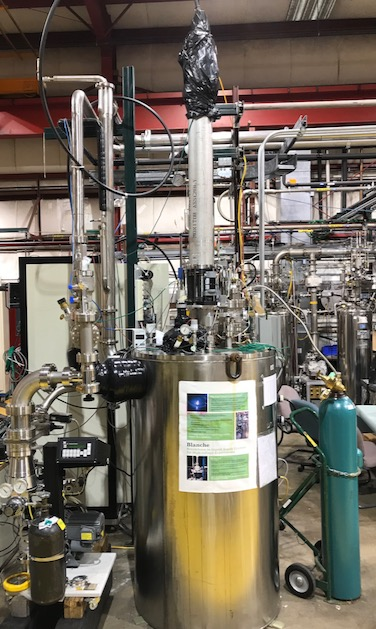
\includegraphics[width=0.35\textwidth]{figures/BlancheCryostat.jpg}%                          
\end{dunefigure}
